\documentclass[a4paper,11pt]{article}
%\usepackage[T1]{fontenc}

%\setlength{\textwidth}{20cm}
%\setlength{\marginparwidth}{0cm}
%\setlength{\voffset}{0cm}
\usepackage[utf8]{inputenc}
\usepackage[francais]{babel}
\usepackage{amsmath}
\usepackage{graphicx}
\usepackage{listings}
%==== to fix locations of figures and tables
\usepackage{float}
\usepackage{placeins}

\lstset{
language=VHDL,
basicstyle=\small\sffamily,
numbers=left,
numberstyle=\tiny,
frame=tb,
columns=fullflexible,
showstringspaces=false
}
%\special{papersize=210mm,297mm}

\title{{\Huge Electronique numérique}\\Décomposition FSMD et Synthèse d'un système numérique}
%\title{TD1}
\date{}

\begin{document}
\maketitle

% ANNEE prochaine ==> load avec registre à décallage
\section{But du TE}

Le but de ce TE est de ``synthétiser'' un circuit numérique sur un FPGA. C'est la première expérience concrète que l'on réalise dans l'UV 1.5 ! \\

Nous allons pour cela procéder de la même manière qu'aux TE précédents, en adjoignant une nouvelle étape dans le processus :

\begin{itemize}
\item Formuler le problème sous forme de {\bf diagramme à bulles}.
\item Etablir les équations logique de notre {\bf contrôleur} \footnote { (ou ``FSM'' ou ``automate'',...)}
\item {\bf Simuler} le circuit virtuel pour s'assurer qu'il fonctionne comme prévu.
\item {\bf Synthétiser} le circuit sur FPGA, et le faire fonctionner ``pour de vrai''.
\end{itemize}

\section{Position du problème : multiplieur séquentiel}

Nous savons qu'il est {\it certes} possible de trouver un circuit purement {\it combinatoire} qui réalise la multiplication...Nous n'allons pas procéder ainsi.\\

Le multiplieur  proposé ici {\it séquentiel} : il lui faudra plusieurs cycles pour réaliser son calcul. L'algorithme de multiplication séquentielle reproduit ce que l'on fait sur papier, lorsqu'on multiplie 2 nombres.\\

Pour multiplier $X$ par $Y$, la methode consiste à cumuler séquentiellement les produits partiels :

$$ P=X \times Y = \sum_{i}Y_i\times X \times 2^i$$

Il est très important de comprendre la signification de cette équation : selon la valeur de $Y_i$, le terme $ (Y_i \times X) \times  2^i $ de rang i de la somme vaut :
\begin{itemize}
\item 0 si Yi = 0 ou
\item X décalé de i positions vers la gauche si $Yi = 1$. Le décallage se fait par $2^i$ !
\end{itemize}


\begin{figure}[!h]
\begin{center}
\includegraphics[scale=0.4]{./figures/algo_mult2.png}
\end{center}
\caption{Principe de la multiplication : une séquence de produits partiels et de décalages}
\end{figure}
%\FloatBarrier

\begin{figure}[!h]
\begin{center}
\includegraphics[scale=0.15]{./figures/flowchart.png}
\end{center}
\caption{Flowchart de l'algorithme de multiplication séquentielle}
\end{figure}
\FloatBarrier

\begin{figure}[!h]
\begin{center}
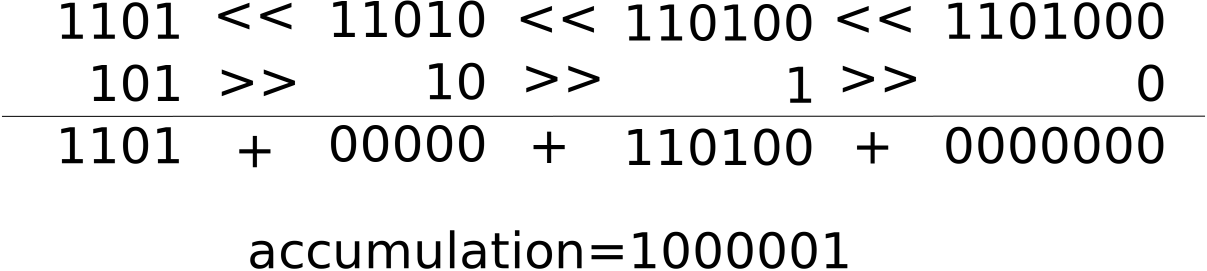
\includegraphics[scale=0.3]{./figures/algo.png}
\end{center}
\caption{Déroulement de l'algorithme de multiplication séquentielle}
\end{figure}
\FloatBarrier
%{\bf Question : } donner les différentes valeurs binaires (et décimales) des registres A, B et ACCU au cours de la multiplication pour $A=5$ et $B=13$.

\section{Décomposition FSMD}

\subsection{Rappels}
La décomposition FSMD (ou contrôleur-chemin de données) est rappelée ici, de manière générique. Le contrôleur réagit aux status du chemin de données, et contrôle ce dernier en conséquence. Le contrôleur réagit également aux ordres extérieurs (dans notre cas un 'start'), en renseigne l'extérieur sur la disponibilité des données produites (dans notre cas un signal 'end' indiquant la disponibilité du calculateur pour un nouveau calcul).

\begin{figure}[!h]
\begin{center}
\includegraphics[scale=0.3]{./figures/FSMD-2.png}
\end{center}
\caption{Chemin de données générique}
\end{figure}
\FloatBarrier

\subsection{Chemin de données}

Les principes d'additions et de décallages successifs nous invitent à considérer 3 registres : regA, regB et ACCU qui contiendront les valeurs de A,B et de l'addition courante.

{\bf Question 1 : }  donner les différentes valeurs binaires (et décimales) des registres regA, regB et ACCU au cours de la multiplication pour $A=5$ et $B=13$.\\

{\bf Question 2 : }  trouver une condition d'arrêt de cet algorithme. Cette condition constituera un élement du {\it status} renvoyé au contrôleur.\\

Le schéma suivant recense ces opérateurs, les registres ainsi que les routages (multiplexeurs) entre ces élements.

\begin{figure}[!h]
\begin{center}
\includegraphics[scale=0.3]{./figures/datapath.png}
\end{center}
\caption{Chemin de données de l'algorithme}
\end{figure}
%\FloatBarrier

{\bf Question 3 :} tenter de donner un nom significatif au signaux de contrôle des différents multiplexeurs.

\subsection{Codage VHDL du chemin de données}


Sous Moodle on donne un code ``à trous'' du chemin de données. Le codage VHDL du registre regA est rappelé ici également.\\

{\bf Question 4 :} analyser ce code en tentant de faire la correspondance avec le schéma du datapath. En particulier, où se trouve le signal ``A\_Reg\_Comb'' ?\\

{\bf Question 5 :} en vous inspirant de ce code, écrire regB, puis celui d'ACCU. Pour ce dernier, vous aurez besoin d'additionner. Le type {\it unsigned} utilisé ici pour typer les registres permet effectivement d'additionner (ce n'est logiquement pas le cas de vecteurs de bits).\\

\begin{lstlisting}[caption=registre A et logique combinatoire associée, label=amb]
 a_reg_proc : process (clk, reset_n)
  begin
    if reset_n = '0' then
      reg_a <= "0000";
    elsif rising_edge(clk) then
      reg_a <= reg_a_comb;
    end if;
  end process;

  reg_a_comb <= unsigned(a) when chRa = '1' else
                '0' & reg_a(3 downto 1) when shift = '1' else
                reg_a;
\end{lstlisting}


\subsection{Conception de l'automate}

Le diagramme à bulle de l'automate est donné ici. Les premiers états servent à attendre la fourniture des opérandes $A$ et $B$ : la présence de ces données est signalée respectivement par des signaux externes $ack_A$ et $ack_B$.

\begin{figure}[!h]
\begin{center}
\includegraphics[scale=0.4]{./figures/controleur_fsm.png}
\end{center}
\caption{Contrôleur de l'algorithme}
\end{figure}
\FloatBarrier

{\bf Question 6 :} établir les équations de cet automate afin de contrôler le chemin de données précédent.\\

{\bf Question 7 :} remplir le code à trou concernant ce contrôleur, dans le même fichier, à l'endroit prévu pour cela. En ce qui concerne le codage VHDL, inspirez vous du TE3.\\

\section{Simulation}

Un banc de test vous est fourni sous Moodle, qui teste le produit de $5$ par $15$.\\

{\bf Question 8 :} avec GHDL, analyser puis simuler votre circuit.

\section{Synthèse FPGA}

Lorsque vous avez simulé correctement, consultez votre enseignant pour observer le circuit synthétisé sur un FPGA (FPGA de la société Xilinx, sur carte Nexys 2 de la société Digilent).

\end{document}
